% ----------------------------------------------------------------
% Article Class (This is a LaTeX2e document)  ********************
% ----------------------------------------------------------------
\documentclass[12pt]{article}
\usepackage[a4paper,top=2.5cm, bottom=2.5cm, left=2cm , right=2cm]{geometry}
\usepackage[english]{babel}
\usepackage{amsmath,amsthm}
\usepackage{amsfonts}
\usepackage{multirow}
\usepackage{color,ulem}
\usepackage{graphicx}
\usepackage{enumitem}
\usepackage[round]{natbib}
\usepackage{makeidx}
  \makeindex
\usepackage[hidelinks]{hyperref}
%\AtBeginDocument{\let\textlabel\label} % When problem with \label in align environment
%\usepackage{mdframed}
\usepackage[framemethod=TikZ]{mdframed}
  \mdfdefinestyle{MyFrame}{%
    linecolor=blue,
    outerlinewidth=1pt,
%    roundcorner=20pt,
%    innertopmargin=\baselineskip,
    innertopmargin=3pt,
%    innerbottommargin=\baselineskip,
%    innerrightmargin=20pt,
%    innerleftmargin=20pt,
%    backgroundcolor=gray!50!white
    }
% THEOREMS -------------------------------------------------------
\newtheorem{thm}{Theorem}[section]
\newtheorem{cor}[thm]{Corollary}
\newtheorem{lem}[thm]{Lemma}
\newtheorem{prop}[thm]{Proposition}
\theoremstyle{definition}
\newtheorem{defn}[thm]{Definition}
\newtheorem{assum}[thm]{Assumption}
\theoremstyle{remark}
\newtheorem{rem}[thm]{Remark}
\numberwithin{equation}{section}

\usepackage{mhchem}
\newcommand{\reactionRev}[4]{#1 \ce{<=>[#3][#4]} #2}
\newcommand{\reactionIrr}[4]{#1 \ce{->[#3][#4]} #2}

\graphicspath{{figures/}}

% ----------------------------------------------------------------
\begin{document}
\normalem

\title{{IMSV}: bacteria simulator design \\ Version 0.0}%
\author{M.~Dinh and S.~Fischer}%
%\address{er}%
%\thanks{zq}%
\date{\today}%

\newpage

\tableofcontents

\newpage

\section{Introduction}

The aim of this document is not to go into technical details of the implementation (the code is documented using Doxygen, technical details are therefore best found in the Doxygen-generated manual). Rather we wish to walk through the choices in design that have been made. The technical manual hopefully contains necessary information for understanding the concept behind each class and how to use it. However it does not tell you what classes are central in the architecture and it is difficult to see at a glimpse how classes interact.

Describing global design should be more agreeable to read than the purely technical document. It helps understand how we tackled a certain number of efficiency issues (should it be speed or maintainability). Most efficiency issues in programming are related to architecture design rather than class implementation. Efficiency of an architecture can be related to information flowing between classes. Restricting information access through classes and dependencies between classes is generally considered good style, as it limits data corruption and enhances maintainability. Achieving this increases the probabilities that the simulator behaves the way it should and facilitates further expansions.

Once data protection and maintainability are ensured, speed issues are addressed only if they can be identified. Most parts of the simulator are not critical in that regard and do not need a particularly refined design or implementation. If speed issues arise, two level of solutions can be worked on. At the lowest level, class implementations can be changed to perform some routines more quickly (generally leading to at most a couple-fold speed increase). At the highest level, communication between classes can be tuned to ensure that only the necessary computations are done (generally leading to a drastic speed increase and a complexification of the architecture with new classes that "filter" communications).

To sum up, description at a global level gives critical insight into how the simulator works and where speed/design issues have been identified during development. It should facilitate discussions even with non-programmers (or at least non-C++-programmers).

\section{Reactant hierarchy}

\subsection{UML class diagram}

\begin{figure}[!ht]
	\centering
	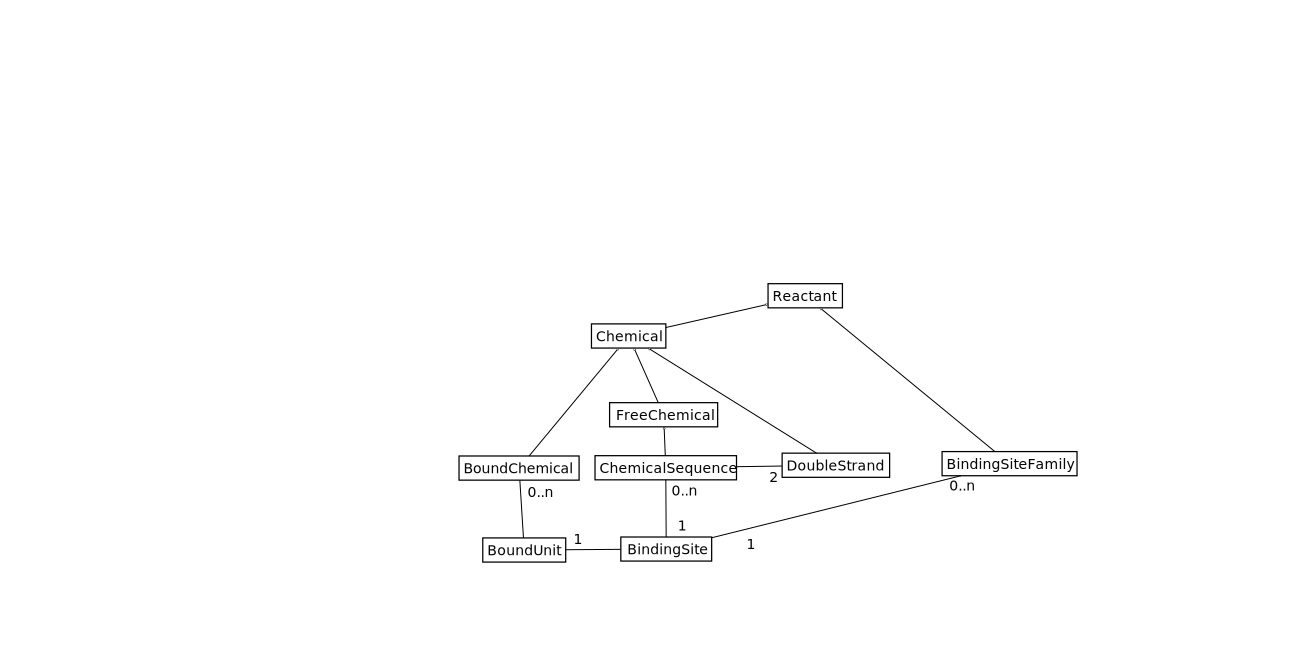
\includegraphics[width=0.8\linewidth]{reactant_uml}
\end{figure}

\subsection{Reactant}

\texttt{Reactant} is a global abstract interface. All entities that can participate in a reaction \emph{must} inherit from it.

\subsection{Chemical}

\begin{figure}[!ht]
	\centering
	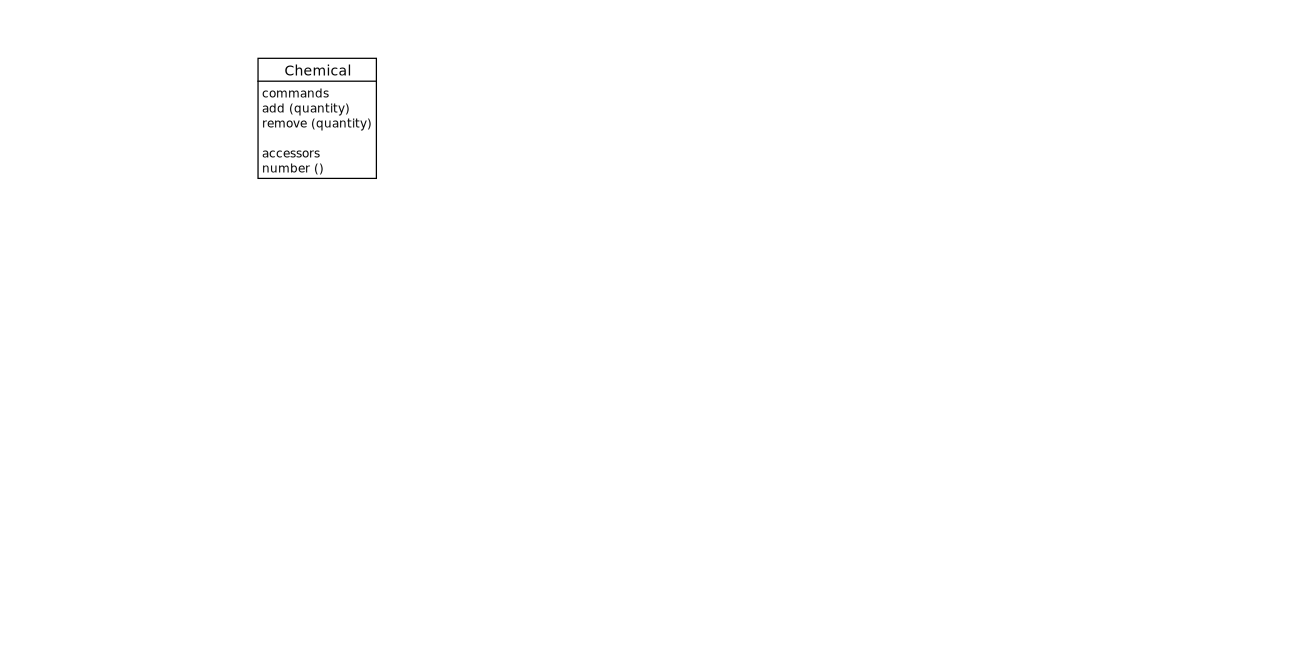
\includegraphics[scale=0.8]{chemical}
\end{figure}

\texttt{Chemical} defines all standard chemical entities. Instances of the class (as opposed to instances of subclasses) are considered to be free chemical (\textit{e.g.} molecules diffusing in the cytosol or extracellular medium). \texttt{Chemical} represents a \emph{pool} of a given chemical species, meaning that one can add/remove a given quantity of it, and access its current number at any time.

\paragraph{Input format}
\begin{verbatim}
unit Chemical <name> [<initial quantity>]
\end{verbatim}

\subsection{BoundChemical}

\begin{figure}[!ht]
	\centering
	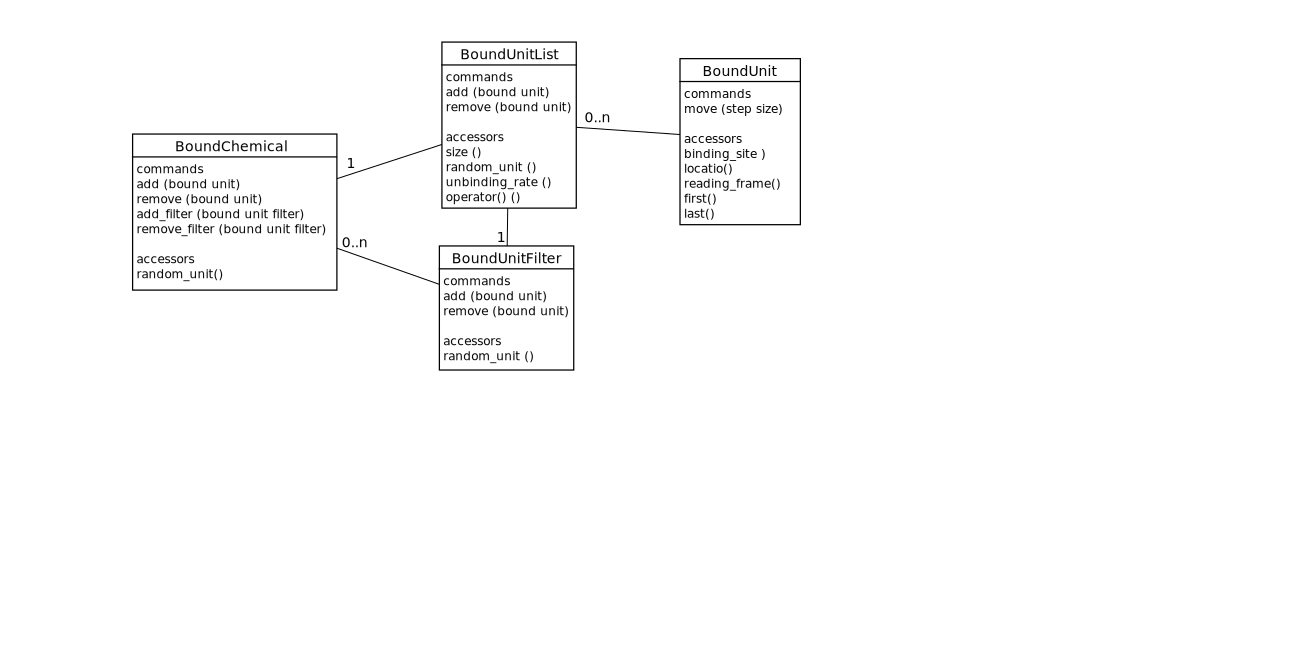
\includegraphics[scale=0.8]{boundchemical}
\end{figure}

\texttt{BoundChemical} is a subclass of \texttt{Chemical} that represents chemicals that are bound to a sequence. It is important to note it only represents molecules bound to the sequence, \emph{not} the complex formed by the chemical and the sequence. Even though \texttt{BoundChemical} represents a pool of molecules, single elements are not interchangeable, they are defined by their position on a sequence. \texttt{BoundChemical} uses two classes \texttt{BoundUnit} and \texttt{BoundUnitList} to represent molecules individually. An external user cannot access the latter directly, he can only focus a random unit of the pool.

\paragraph{Input format}
\begin{verbatim}
unit BoundChemical <name>
\end{verbatim}

\subsection{ProcessiveChemical}

\begin{figure}[!ht]
	\centering
	\includegraphics[scale=0.8]{processivechemical}
\end{figure}

\texttt{ProcessiveChemical} is a subclass of \texttt{BoundChemical}. Compared to a standard \texttt{BoundChemical}, it is able to move along the sequence and recognize a termination site. A stalled form is associated with it. It is used when the chemical meets a termination site or the end of the sequence and cannot move anymore.

\paragraph{Input format}
\begin{verbatim}
unit ProcessiveChemical <name> <stalled form> <termination site>
\end{verbatim}


\subsection{Loader}

\begin{figure}[!ht]
	\centering
	\includegraphics[scale=0.8]{loader}
\end{figure}

\texttt{Loader} is a subclass of \texttt{BoundChemical}. Compared to a standard \texttt{BoundChemical}, it is able to read templates on the sequence and load elements matching the sequence. The template element matching is done using a \texttt{DecodingTable}, which also specifies the state of the loader in its occupied form (when an element has effectively been loaded on its template) and the loading rate for every template-element pair.

\paragraph{Input format}
\begin{verbatim}
unit Loader <name> <decoding table>
unit DecodingTable <name> \
  [<template> <element to load> <element-loader complex> <loading rate>]^N
\end{verbatim}


\subsection{ChemicalSequence}

\begin{figure}[!ht]
	\centering
	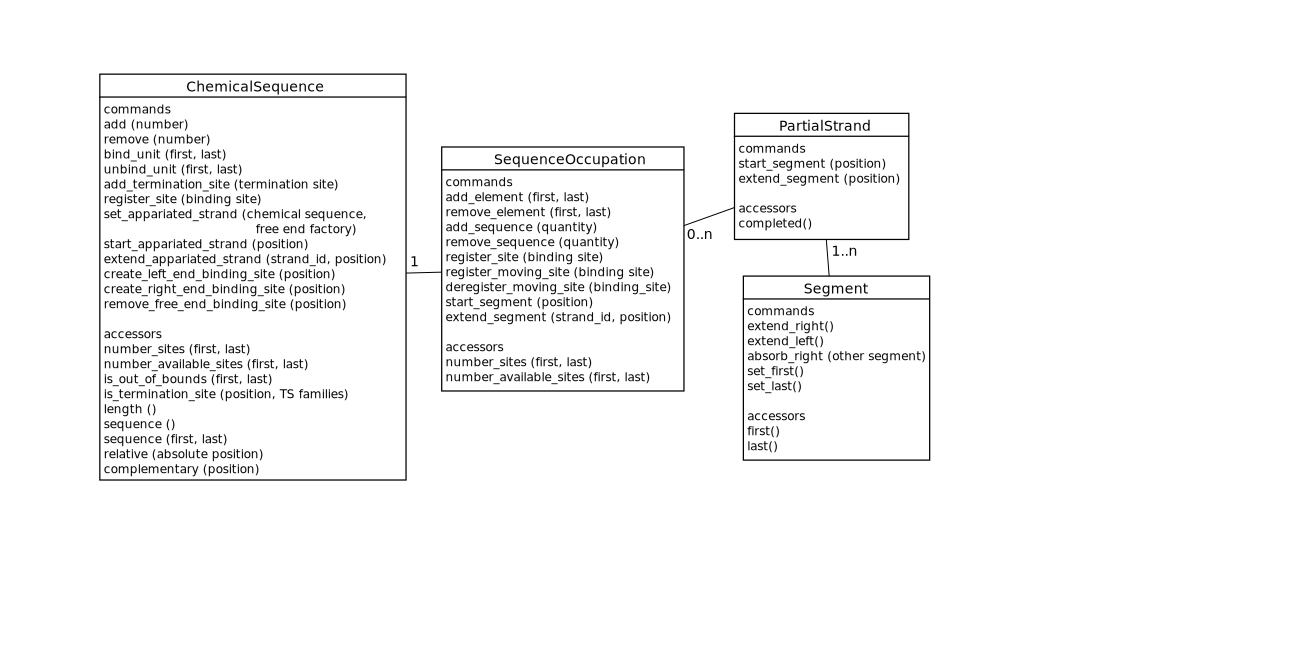
\includegraphics[scale=0.8]{chemicalsequence}
\end{figure}

\texttt{ChemicalSequence} is a subclass of \texttt{Chemical}. It is defined by a sequence and the ability to bind elements (more precisely \texttt{BoundChemical}). However, instances of a sequence are \emph{not} treated individually, it is impossible to tell to which instance a given chemical bound. An object called \texttt{SequenceOccupation} maintains occupation levels at sites of interest. For example, suppose the sequence is an mRNA carrying a ribosome binding site for the protein DnaA. The number of available sites is obtained by removing the number of bound chemicals occupying the site from the number of instances of the mRNA currently in the cell.

\paragraph{Input format}
\begin{verbatim}
unit ChemicalSequence <name> sequence <sequence> [<initial quantity>]
unit ChemicalSequence <name> product_of <parent sequence> \
  <starting position> <ending position> <product table> [<initial quantity>]
\end{verbatim}

\subsection{BindingSiteFamily}

\begin{figure}[!ht]
	\centering
	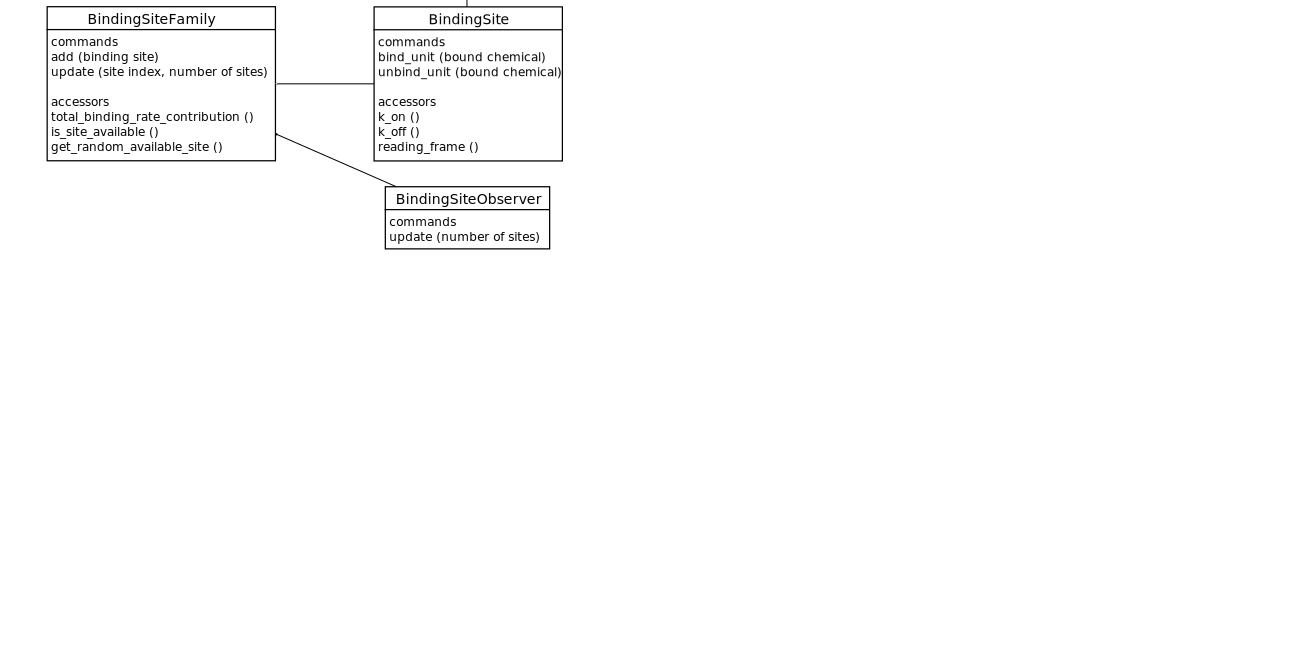
\includegraphics[scale=0.8]{bindingsitefamily}
\end{figure}

\texttt{BindingSiteFamily} is a subclass of \texttt{Reactant}. Contrary to \texttt{Chemical}, it does not represent a countable pool of molecules. Each family contains a number of related instances of \texttt{BindingSite}. A \texttt{BindingSiteObserver} is used to dynamically maintain the number of available sites for each binding site.

\paragraph{Input format}
\begin{verbatim}
unit BindingSite <binding site family name> <chemical sequence> \
  <start> <end> <k_on> <k_off> [<reading frame>]
\end{verbatim}


\section{Reaction hierarchy}

\subsection{UML class diagram}

\begin{figure}[!ht]
	\centering
	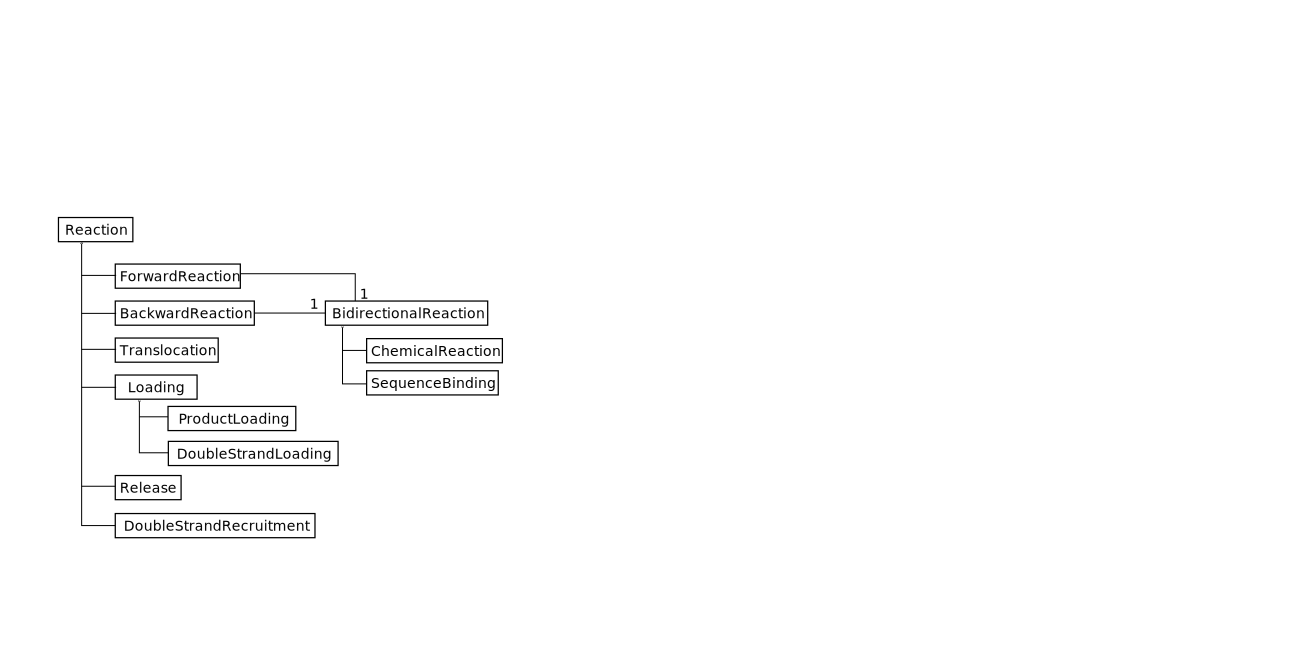
\includegraphics[width=0.8\linewidth]{reaction_uml}
\end{figure}

\subsection{Reaction}

\begin{figure}[!ht]
	\centering
	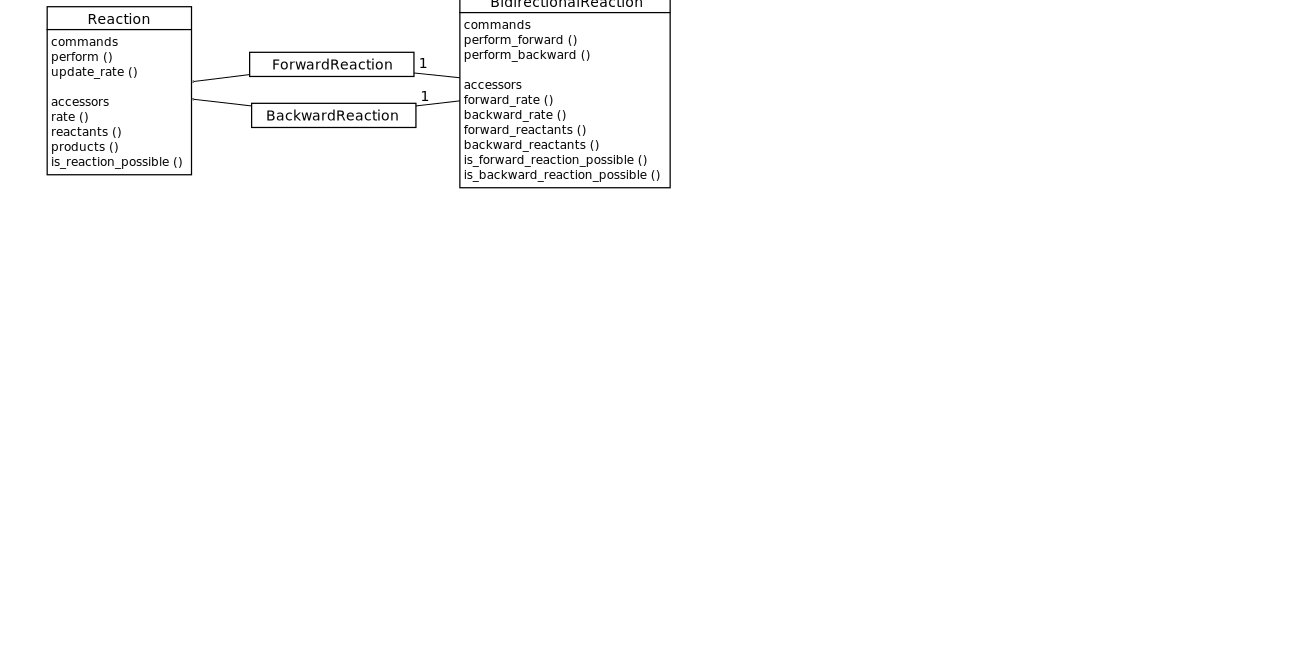
\includegraphics[width=0.8\linewidth]{reaction}
\end{figure}

There are two abstract classes used to define reactions: \texttt{Reaction} for one-way reactions and \texttt{BidirectionalReaction} for reversible reactions. Two adapter classes \texttt{ForwardReaction} and \texttt{BackwardReaction} split reversible reactions in two one-way reactions. In the end, the solver only handles one-way reactions. A reaction can necessarily be performed, its rate updated and accessed and is composed of reactants and products.

\subsection{ChemicalReaction}


\paragraph{Input format}
\begin{verbatim}
reaction ChemicalReaction [<chemical> <stoichiometry>]^N rates <k_1> <k_-1>
\end{verbatim}

\paragraph{Formula} A \texttt{ChemicalReaction} represents association/dissociation of an arbitrary number of elements. It is defined by
$$
	\reactionRev{a_1 A_1 + a_2 A_2 + ... + a_r A_r}{b_1 B_1 + ... + b_p B_p}{k_1}{k_{-1}}
$$
where
\begin{itemize}
	\item $A_i$ and $B_i$ are of type \texttt{Chemical}. They \emph{must not} be of type \texttt{BoundChemical}, \emph{except} if there is exactly one \texttt{BoundChemical} on each side of the equation. 
	\item $a_i$ and $b_i$ are stoichiometric coefficients.
	\item $k_1$ and $k_{-1}$ are rate constants.
\end{itemize}

\paragraph{Action} When the reaction is performed, the number of chemicals involved is changed according to their stoichiometric coefficient. If \texttt{BoundChemical} are involved, the simulator will assume that the bound chemical that is consumed is replaced by the bound chemical on the other side of the equation (\textit{i.e.} it will be bound at the location previously occupied by the precursor).

\paragraph{Rate} The rates are given by
$$
	\lambda_{forward} = k_1 \prod\limits_{i=1}^{r} [A_i]^{a_i}
$$
$$
	\lambda_{backward} = k_{-1} \prod\limits_{i=1}^{p} [B_i]^{b_i}
$$

\subsection{Complexation}
\paragraph{Input format}
\begin{verbatim}
reaction Complexation [<chemical> <stoichiometry>]^N rates <k_1> <k_-1>
\end{verbatim}

\paragraph{Formula} A \texttt{Complexation} represents association/dissociation of two elements. It is defined by
$$
	\reactionRev{A + B}{C}{k_{on}}{k_{off}}
$$
where
\begin{itemize}
	\item $A$, $B$ and $C$ are of type \texttt{Chemical}. They \emph{must not} be of type \texttt{BoundChemical}, \emph{except} if there is exactly one \texttt{BoundChemical} on each side of the equation. In the latter case, the simulator will assume that the bound chemical that is consumed is replaced by the bound chemical on the other side of the equation (\textit{i.e.} it will be bound at the location previously occupied by the precursor).
	\item $k_{on}$ and $k_{off}$ are rate constants.
\end{itemize}

\paragraph{Action} When the reaction is performed, the number of chemicals involved is increased/decreased by 1. If \texttt{BoundChemical} are involved, the simulator will assume that the bound chemical that is consumed is replaced by the bound chemical on the other side of the equation (\textit{i.e.} it will be bound at the location previously occupied by the precursor).

\paragraph{Rate} The rates are given by
$$
	\lambda_{forward} = k_{on} [A][B]
$$
$$
	\lambda_{backward} = k_{off} [C]
$$

\subsection{SequenceBinding}
\paragraph{Input format}
\begin{verbatim}
reaction SequenceBinding <chemical> <bound form> <binding site family>
\end{verbatim}

\paragraph{Formula} A \texttt{SequenceBinding} represents binding of a free element on a binding site of a sequence. It is defined by
$$
	\reactionRev{C_{free} + BSF}{C_{bound}}{}{}
$$
where
\begin{itemize}
	\item $C_{free}$ is of type \texttt{Chemical} but not \texttt{BoundChemical}.
	\item $BSF$ is of type \texttt{BindingSiteFamily}.
	\item $C_{bound}$ is of type \texttt{BoundChemical}.
\end{itemize}

\paragraph{Action} When the forward reaction is performed, a random available binding site is drawn from the binding site family (drawing is weighted by affinity). A $C_{free}$ molecule is removed from the pool and a $C_{bound}$ added to the \texttt{ChemicalSequence} bearing the binding site. When the backward reaction is performed, a random molecule of $C_{bound}$ is removed from the pool (and from its sequence) and a $C_{free}$ molecule is added.

\paragraph{Rate} The rates are given by
$$
	\lambda_{forward} = \frac{[C_{free}]}{V_c} \sum_{\text{sites }s \in BSF} (k_{on})_s \times \text{Number of sites $s$ available}
$$ 
$$
	\lambda_{backward} = \frac{1}{V_c} \sum_{\text{molecules }m \in C_{bound}} (k_{off})_\text{site on which $m$ is bound}
$$
\begin{itemize}
	\item $(k_{on})_s$ is the association constant of $C_{free}$ with binding site $s$.
	\item $(k_{off})_s$ is the dissociation constant of $C_{bound}$ with binding site $s$.
	\item $V_c$ is the volume of the cell.
\end{itemize}

\subsection{Translocation}
\paragraph{Input format}
\begin{verbatim}
reaction Translocation <processive chemical> <form after step> <step size> <rate>
\end{verbatim}

\paragraph{Formula} A \texttt{Translocation} represents movement of a bound element along a sequence. It is defined by
$$
	\reactionIrr{C}{C_\text{after step}}{k}{}
$$
where
\begin{itemize}
	\item $C$ is of type \texttt{ProcessiveChemical}.
	\item $C_\text{after step}$ is of type \texttt{BoundChemical}.
	\item $k$ is a rate constant.
\end{itemize}

\paragraph{Action} When the reaction is performed, a random $C$ is chosen. Generally, it is replaced by a $C_\text{after step}$, moved by a step of a given size along the sequence the original $C$ is bound to. If the chemical cannot move because it reached the end of the sequence or it reaches a termination site, it is replaced by the stalled form of the \texttt{ProcessiveChemical} $C$.

\paragraph{Rate} The rate is given by
$$
	\lambda = k [C]
$$

\subsection{Loading}
\paragraph{Input format}
\begin{verbatim}
reaction Loading <loader>
\end{verbatim}

\paragraph{Formula} A \texttt{Loading} typically represents loading of elements by a polymerase onto a template sequence. It is defined by
$$
	\reactionIrr{L + E}{LE}{}{}
$$
where
\begin{itemize}
	\item $L$ is of type \texttt{Loader}.
	\item $E$ is an element to load, of type \texttt{Chemical} but not \texttt{BoundChemical}. It is defined in $L$'s \texttt{DecodingTable}.
	\item $LE$ is the occupied form of the loader, of type \texttt{BoundChemical}. It is defined in $L$'s \texttt{DecodingTable}.
\end{itemize}

\paragraph{Action} Each instance of $L$ reads a specific template. Using its \texttt{DecodingTable}, we know which $E$ it tries to load, which $LE$ is yielded if loading occurs and the loading rate associated with the template. When the reaction is performed, a random $L$ is chosen according to loading rates. An element to load $E$ is removed from the pool and $L$ is replaced with $LE$.

\paragraph{Rate} The rate is given by
$$
	\lambda = \sum_{t\in templates} k_t[L_t][E_t]
$$
where
\begin{itemize}
	\item $k_t$ is the loading rate associated with template $t$.
	\item $L_t$ corresponds to loaders $L$ reading template $t$.
	\item $E_t$ is the chemical to load onto template $t$.
\end{itemize}

\subsection{Release}
\paragraph{Input format}
\begin{verbatim}
reaction Release <bound chemical> [<chemical> <stoichiometry>]^N rate <rate> \
  [produces <product table>]
\end{verbatim}

\paragraph{Formula} A \texttt{Release} represents detachment of a bound element from a sequence. An arbitrary number of elements can be used as coreactants to trigger the release, and an arbitrary number of products are released. It is defined by
$$
	\reactionIrr{B + a_1 A_1 + ... + a_r A_r}{\delta_PP + c_1 C_1 + ... + c_p C_p }{k}{}
$$
where
\begin{itemize}
	\item $B$ is of type \texttt{BoundChemical}.
	\item $P$ is of type \texttt{ChemicalSequence}. It is a product that is released if $B$ is a polymerase. In the latter case $\delta_P = 1$ else $\delta_P = 0$.
	\item $A_i$ are of type \texttt{Chemical}, but not \texttt{BoundChemical}.
	\item $C_i$ are of type \texttt{Chemical}, but not \texttt{BoundChemical}.
	\item $a_i$ and $c_i$ are stoichiometric coefficient.
	\item $k$ is a rate constant.
\end{itemize}

\paragraph{Action} When the reaction is performed, a random $B$ is chosen and removed from the pool (and detached from its sequence). The $A_i$ and $C_i$ pool are changed according to their stoichiometric coefficients. If a product table is defined, it means that the released chemical is a polymerase. A product (a chemical sequence) corresponding to the bound chemical's binding and release points is added.

\paragraph{Rate} The rate is given by
$$
	\lambda = k[B]\prod\limits_{i=1}^{r}[A_i]^{a_i}
$$

\subsection{Degradation}
\paragraph{Input format}
\begin{verbatim}
unit CompositionTable <name> <letter_1> [<chemical>]^N
...
unit CompositionTable <name> <letter_N> [<chemical>]^N

reaction Degradation <chemical sequence> <composition table> <rate>	
\end{verbatim}

\paragraph{Formula} A \texttt{Degradation} represents decomposition of a sequence into base components. It is defined by
$$
	\reactionIrr{CS}{b_1 + b_2 + ... + b_N}{k}{}
$$
where
\begin{itemize}
	\item $CS$ is of type \texttt{ChemicalSequence}.
	\item $b_i$ are of type \texttt{Chemical}, but not \texttt{BoundChemical}. They are found in a \texttt{CompositionTable} specified in the reaction.
	\item $k$ is the degradation constant.
\end{itemize}

\paragraph{Action} When the reaction is performed, a $CS$ is removed from the pool. A \texttt{CompositionTable} is specified along the reaction. It allows base-by-base conversion of the sequence of $CS$ into components yielded by degradation. The pools of base components is updated accordingly. In the simulator, a degradation reaction is effectively implemented as a \texttt{ChemicalReaction}.

\paragraph{Rate} The rate is given by
$$
	\lambda = k [CS]
$$


\section{Solver hierarchy}


\end{document}
% ----------------------------------------------------------------
